
\chapter{HARDroid: Reconocedor de Actividades Humanas}

\label{chap5:hardroid}

\section{Introducción}

\label{sec51:intro}En este capítulo introducimos un sistema que clasifica
la actividades humanas ambulatorias utilizando teléfonos móviles inteligentes
con la plataforma \abbr{Android}\texttrademark: \emph{HARDroid}.
El sistema es una adaptación del diseño utilizado por sistemas existentes
como \emph{Google Play Services} \cite{Google2013l}, específicamente
la funcionalidad para reconocer actividades humanas utilizando los
conceptos y técnicas expuestos en capítulos precedentes. 

El sistema \emph{HARDroid} está implementado en base a dos componentes
principales: una interfaz de programación que expone las facilidades
y un servicio en ejecución que realiza las funciones principales del
sistema. La interfaz para programadores (\abbr{API}) proporciona
una firma de funciones bien definidas junto con la documentación adecuada
para que toda aplicación móvil de terceros utilice como un componente
externo la solución de un sistema \abbr{HAR}. El servicio de trasfondo
en la plataforma \abbr{Android} es una aplicación para teléfonos
móvil independiente que implementa algoritmos de reconocimiento de
actividades humanas.

La propuesta de este trabajo se basa en un diseño desacoplado para
contar con una implementación genérica y extensible de un sistema
\abbr{HAR}. Como en todo sistema de \emph{software}, el diseño adecuado
posibilita la evolución y mantenimiento del mismo sin afectar el funcionamiento
de otras aplicaciones móviles clientes dependientes. 

Las siguientes secciones se organizan de la siguiente manera: primeramente
en la sección \ref{sec52:dise=0000F1o} damos una introducción de
las consideraciones de diseño y metodología utilizadas para la construcción
de los componentes de software. Se empieza con los conceptos generales
de Ingeniería de Software hasta concluir con los detalles técnicos
de la plataforma \abbr{Android}. La siguiente sección \ref{sec53:arquitectura}
incluye una vista general del sistema explicando su arquitectura.
La sección \ref{sec54:hardroid} conforma el núcleo principal de este
proyecto donde una implementación \abbr{HAR} en forma de aplicación
móvil desacoplado es presentado. También, en la sección \ref{sec55:activity}
se explica el desenvolvimiento de una herramienta para realizar experimentos
y evaluar los resultados asociados a la solución. Por último, en la
sección \ref{sec56:conclusion} se discuten los resultados preliminar
obtenidos como motivo de los componentes de software construidos.

\section{Diseño General}

\label{sec52:dise=0000F1o}La construcción del sistema \emph{HARDroid
}está enmarcado dentro del ecosistema de aplicaciones móviles. Desde
el punto de vista conceptual del desarrollo de aplicaciones móviles
es necesario enfocarse en dos aspectos principales para el diseño:
el medio y el contexto.

Una aplicación móvil puede presentarse en diversos medios que corresponden
con el enfoque técnico \cite{Fling2009}, es decir: un sitio Web Móvil,
una aplicación Web Móvil, SMS, Juegos, controles utilitarios\footnote{\emph{Widgets}}
y aplicaciones nativas. Las aplicaciones nativas son uno de los medios
más utilizados debido a la rica experiencia de usuario y capacidades
que pueden ser explotadas en los dispositivos, ya que disponen de
gran soporte en la plataforma subyacente. Por ejemplo, en la plataforma
para teléfonos móviles \abbr{Android}\emph{ }se dispone de las capacidades
disponibles del dispositivo como almacenamiento, ubicación, sensores
y además un medio de distribución certificado como ser el \emph{Google
Play Store} \cite{Google2016p}. 

Por otro lado, está el contexto de la aplicación que se refiere a
la experiencia que el usuario final obtiene al utilizar el sistema
móvil. Para esto el sistema móvil procesa la información de contexto
que rodea al usuario dando una interacción distinta a los sistemas
convencionales. A continuación se listan los tipos de contexto comunes
utilizados en las aplicaciones móviles y un breve ejemplo de su funcionalidad
\cite{Fling2009}:
\begin{itemize}
\item \emph{Utilidad}: Calculadora, Conversión de monedas.
\item \emph{Localización}: Mapas, Registro de actividades físicas.
\item \emph{Informativo}: Buscar información relevante.
\item \emph{Productividad}: Comprar productos y pagar servicios
\item \emph{Inmersión}: Juegos 
\end{itemize}
Estos tipos de contexto se pueden combinar para crear mejores experiencias
de uso de la aplicación móvil. El trabajo desarrollado en esta tesis
se adecua al modelo de aplicaciones móviles de contexto. Se busca
proveer un componente de \emph{Utilidad} que puede ser combinado con
diferentes aplicaciones móviles desarrollados por terceros y pueda
ser mantenido de forma colaborativa. 

\subsection{Criterios de diseño}

\label{ssec52:criterios-dise=0000F1o}La implementación de este trabajo,
así como la mayoría de los sistemas de información, se rige bajo el
principio de diseño \emph{basado en componentes} donde se busca separar
la complejidad de un sistema en módulos y que estos interactúen entre
sí. Los módulos en el diseño de sistemas mejoran la flexibilidad y
comprensión mientras se reduce el tiempo de desarrollo de los mismos
\cite{Parnas1972}.

Una de las técnicas más comunes de diseño de sistemas\emph{ }es la
separación por capas (\emph{Layering}, en inglés\emph{)} para dividir
un sistema complejo \cite{Fowler2002} en diferentes niveles. 

\subsubsection{Arquitecturas en capas}

Cuando un sistema se construye en términos de capas, los módulos se
organizan en niveles apilados como en un pastel, donde cada capa se
soporta sobre la capa baja subyacente. En este sentido, la capa superior
utiliza varios servicios definidos en capas inferiores, pero la capa
inferior desconoce y no depende de las capas en niveles superiores.
Las capas definen concretamente las responsabilidades y encapsulan
las funcionalidades soportadas en cada nivel.

La popularidad de la división de sistemas en módulos por capas se
volvió más relevante con el auge de los sistemas tipo \emph{Cliente-Servidor}.
Estos sistemas fueron inicialmente concebidos como de dos (2) capas:
el cliente se encarga de la interfaz de usuario y la lógica de la
aplicación, y el servidor usualmente es una bases de datos relacional.
En la \figref{fig5:cliente_servidor} se muestra una representación
de la arquitectura en dos capas. Para sistemas sencillos que desplieguen
información y actualicen datos, este modelo es el más adecuado. Sin
embargo, a medida que se construyen sistemas más complejos, el problema
radica mantener la lógica central del sistema: las reglas de negocio,
validaciones, cálculos, etc. El modelo de dos capas propone ubicar
la lógica central embebida en la interacciones de la Interfaz de Usuario,
la capa cliente, o almacenar los mismos en procedimientos almacenados
en la basa de datos, la capa servidor.

\begin{figure}[H]
\begin{centering}
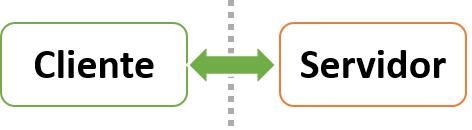
\includegraphics[width=0.8\columnwidth]{capitulo-5/graphics/cliente_servidor}
\par\end{centering}
\caption[Modelo de dos capas]{\label{fig5:cliente_servidor}Modelo de dos capas}
\end{figure}

Debido a las limitaciones del enfoque Cliente-Servidor, se puede extender
el mismo con la ayuda del paradigma de Orientación a Objetos para
construir sistemas con arquitecturas de tres (3) capas. Estas capas
son comúnmente conocidas como \cite{Fowler2002}: Presentación, Dominio
y Recursos. En la \tabref{tab5:tres_capas} se definen las responsabilidades
correspondientes a cada capa. 

\begin{table}[H]
\begin{centering}
\begin{tabular}[t]{|l|>{\raggedright}p{0.5\columnwidth}|}
\hline 
Capa & Responsabilidades\tabularnewline
\hline 
\hline 
Presentación & Provisión de servicios a sistemas externos, despliegue de información
e interacción con el usuario.\tabularnewline
\hline 
Dominio & \multirow{1}{0.5\columnwidth}{Lógica y procesamiento del sistema.}\tabularnewline
\hline 
Recursos & Comunicación con bases de datos, sistemas externos, integración, transacciones
y otros componentes.\tabularnewline
\hline 
\end{tabular}
\par\end{centering}
\caption[Modelo de tres capas]{\label{tab5:tres_capas}Modelo de tres capas}
\end{table}

Independientemente del tipo de sistema de información a ser construido
dividir el mismo en capas lógicas, dividir el sistema en partes separadas,
permite reducir el acoplamiento entre diferentes módulos, inclusive
si todos los módulos se ejecutan en la misma máquina física. En la
\figref{fig5:tres_capas} se muestra la arquitectura de tres capas
discutida anteriormente.

\begin{figure}[H]
\begin{centering}
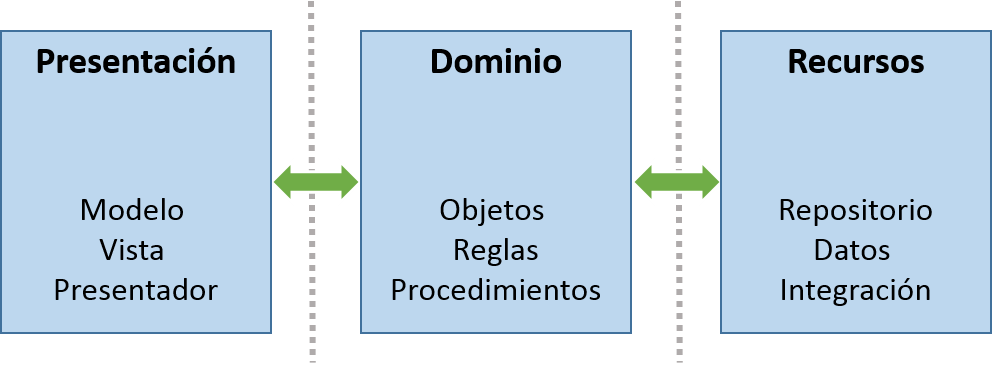
\includegraphics[width=0.8\columnwidth]{capitulo-5/graphics/arqui_tres_capas}
\par\end{centering}
\caption[Modelo de tres capas]{\label{fig5:tres_capas}Modelo de tres capas}

\end{figure}


\subsubsection{Patrones de diseño}

Los patrones de diseño son concepto importante del paradigma de orientación
a objetos, que han sido ideados para solucionar problemas comunes
determinados en un contexto particular \cite{Shalloway2004}. Una
definición acertada es la que se cita a continuación.
\begin{quotation}
<<\emph{Cada patrón describe un problema que ocurre una y otra vez
en nuestro entorno, y también describe la solución principal al problema,
de tal manera que la solución pueda ser utilizada millares de veces,
sin tener que duplicar el trabajo de pensar cómo resolver el problema.>>}
\cite{Alexander1977}
\end{quotation}
Para nuestro objetivo de diseño se utilizan los siguientes patrones
de diseño para organizar la capa de \emph{Dominio} cuya responsabilidad
es la lógica principal del sistema. Se sigue la técnica de dividir
la capa de\emph{ Dominio} por medio de los siguientes patrones \cite{Fowler2002}:
\begin{enumerate}
\item \emph{Service Layer}: Capa de servicios
\item \emph{Domain Model}: Modelo del dominio
\end{enumerate}
La capa de servicios es el punto de interacción entre la \emph{Presentación}
y el\emph{ Dominio}, por lo que actúa como proveedor de una interfaz
clara (comúnmente una \abbr{API} de programación). Este patrón define
los límites del sistema con una capa de servicios que establece el
conjunto de operaciones disponibles y coordina el proceso de cada
operación. La capa de servicios puede ser tan gruesa o tan fina como
se requiera, puede contener objetos de servicio con reglas de negocio,
manejo de transacciones y seguridad.

Por otro lado, el modelo del dominio da soporte a la capa de servicios.
Este patrón define objetos de dominio que tienen incorporados datos
y comportamiento, estos representan de manera significativa el dominio
del problema a resolver. Debido a que la lógica de negocio de un sistema
puede ser bastante compleja, estos objetos están diseñados para manejar
las diversas combinaciones de reglas y lógica del sistema.

\subsubsection{Guías Generales}

En este trabajo fueron utilizadas las guías generales para construcción
de sistemas orientados a objetos. Algunos de los principios más relevantes
que han sido considerados durante el diseño de nuestra solución son
\cite{Albin2003}:
\begin{itemize}
\item Modularidad
\item Orientación a Objetos
\item Reusabilidad
\item Ocultamiento de Información
\item Abstracción
\end{itemize}
Siguiendo estos principios se ha logrado una implementación exitosa
de los componentes y aplicaciones móviles clientes de verificación.
Además, se ha enfocado el desarrollo con miras a la colaboración basada
en la comunidad de código abierto por medio de una Licencia Pública
Apache, Versión 2.0 (\emph{Apache License Version 2.0}, en inglés)
\cite{GimenezYegros2016c}.

\subsection{Metodología de desarrollo}

\label{ssec52:metodologia}En toda labor de construcción de sistemas
de información es necesario definir una metodología de diseño para
encarar problemas y tecnologías complejas. La metodología utilizada
en este trabajo es el diseño descendente (\emph{top-down desing}),
que permite organizar el diseño del sistema en niveles de abstracción
para reducir la complejidad general del sistema \cite{Albin2003}. 

En esta metodología se empieza definiendo la funcionalidad esperada
del sistema como lo requiere el cliente, la capa más alta, y sigue
paso a paso hasta refinar el diseño en capas más bajas a medida que
se avanzan con detalles específicos. 

El diseño empieza poniendo énfasis en las funcionalidades esperadas
del sistema cuando este se encuentre en operación. Luego, se continua
con el diseño de la lógica de negocios que soportan a estas funcionalidades,
y por ultimo se enfoca en los recursos necesarios por la capa lógica.

Como aspecto práctico de esta metodología se han identificado las
siguientes tareas específicas de diseño que ayudan a comprender y
describir mejor el desarrollo de este trabajo:
\begin{enumerate}
\item Diseñar la arquitectura de la solución.
\item Diseñar la capa de servicios, o interfaz del sistema enfocada para
programadores (\abbr{API}) con un conjunto de llamadas a exponer.
\item Diseño de los recursos que conforman el dominio al servicio.
\item Implementación del servicio reconocedor.
\item Implementación de un componente de evaluación de la solución.
\end{enumerate}
Parte de la metodología consistió en definir la interfaz del sistema
en base a las mejores prácticas de la industria para aplicaciones
móviles de contexto, utilizando el lenguaje de programación \abbr{Java}
y la tecnología basada en \abbr{Android}. El diseño se basa en implementaciones
existentes \cite{Google2016m} para heredar las buenas prácticas de
programación y obtener la ventaja de familiaridad de la \abbr{API}
para desarrolladores.

\subsection{Tecnología}

\label{ssec52:tecnologia}Esta sección está dedicada a describir la
tecnología utilizada para la implementación del diseño de este trabajo.
Uno de los criterios claves para la selección de teléfonos móviles
inteligentes apropiados para el reconocimiento de actividades, además
de los sensores, es el sistema operativo (abreviado \abbr{OS}) móvil. 

El sistema operativo móvil se encarga del manejo de recursos del dispositivo
y el control de operación de la aplicaciones móviles. Estos sistemas
tiene características similares a los sistemas operativos convencionales
utilizados en las computadoras de escritorio (\abbr{PC}). La función
principal de un sistema operativo es proveer servicios comunes a las
aplicaciones y administrar los recursos de \emph{hardware}. Adicionalmente,
los sistemas operativos móviles están diseñados para el uso eficiente
de energía, debido a las limitaciones de batería, y características
especiales de movilidad. 

En este trabajo se propone una herramienta que está dirigida a los
teléfonos móviles inteligentes basados en \abbr{Android}. En los
siguientes apartados se da una vista general de \abbr{Android} como
plataforma tecnológica de este capítulo.

\subsubsection{Plataforma}

El sistema operativo móvil \abbr{Android} es una plataforma de código
abierto con un entorno de programación de distribución publica, que
además incluye una interfaz de programación (\abbr{API}) completa
con acceso al \emph{hardware} del teléfono y los sensores internos.
Esta facilidad permite que las herramientas de aprendizaje automático
y sus procedimientos puedan ser construidos de manera más simple. 

\abbr{Android} es una plataforma abierta para dispositivos móviles
encabezada por \emph{Google} y la \emph{Open Handset Alliance \cite{OHA2008}}
con el objetivo de innovar en el entorno móvil, mejorando la experiencia
de usuario a un menor costo \cite{Gargenta2014}. El principal aporte
que logró \abbr{Android} es que por primera vez una plataforma abierta
consigue separar el \emph{software} y el \emph{hardware} subyacente.
Esto permite que un gran número diverso de dispositivos ejecuten las
mismas aplicaciones, creando un ecosistema más variado para desarrolladores
y consumidores. 

\subsubsection{Arquitectura}

La plataforma \abbr{Android} está soportada sobre el núcleo (\abbr{Kernel})
de \abbr{Linux} cuyo proyecto al igual es una iniciativa de código
abierto utilizado ampliamente en el ámbito de tecnología de la información
desde hace más de una década. La capa más baja de la arquitectura
hereda las principales funcionalidades esperadas en los sistemas operativos
modernos: portabilidad, seguridad y las capacidades funcionales.

\begin{figure}[H]
\begin{centering}
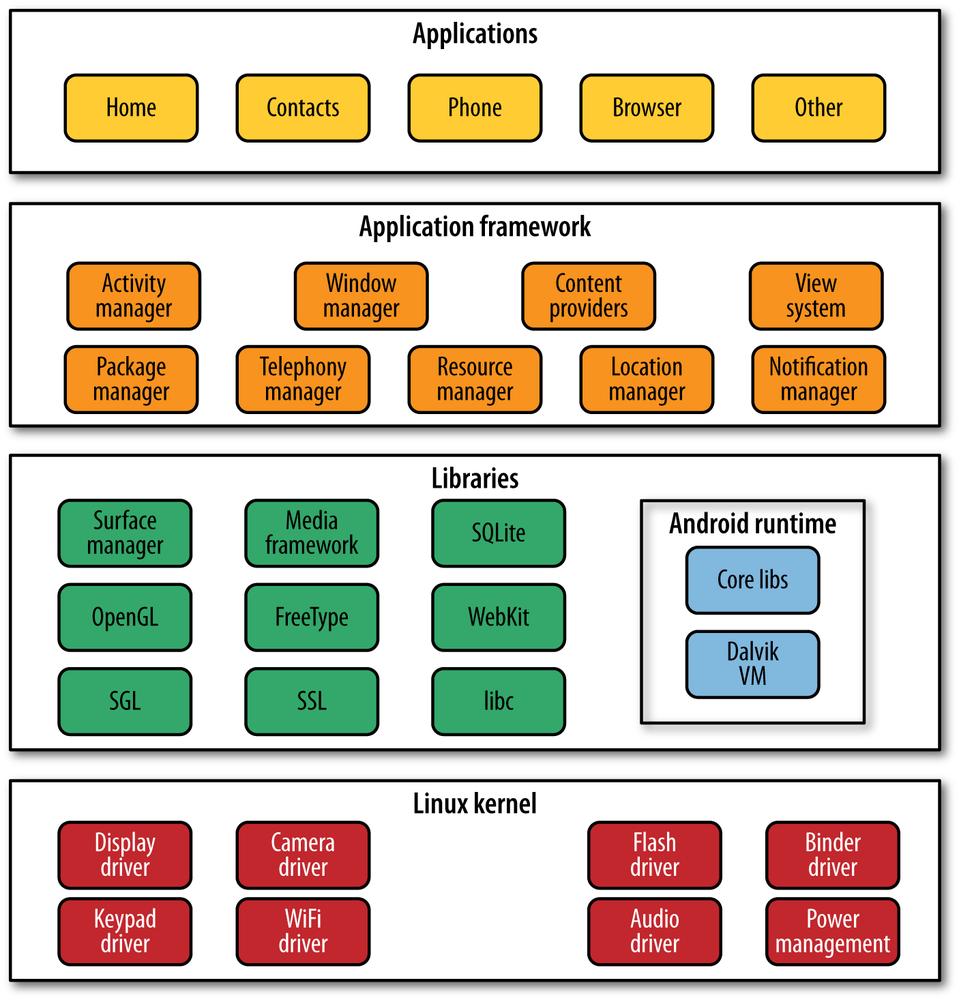
\includegraphics[width=0.8\columnwidth]{capitulo-5/graphics/android_stack}
\par\end{centering}
\caption[Arquitectura de Android]{\label{fig5:android-stack}Arquitectura de \abbr{Android}}
\end{figure}

Adicionalmente, la plataforma ha mejorado el núcleo introduciendo
un número de extensiones especiales para el entorno móvil. Las extensiones
agregan capacidades funcionales mejoradas para administrar la energía;
ya que los móviles utilizan batería, mecanismos para llamados a procedimientos
remotos y aislamiento para mejorar la seguridad \cite{Gargenta2014}.
Las extensiones fueron módulos agregados cuya lista se detalla a continuación
con su nomenclatura en inglés \cite{Schreiber2011}: 
\begin{itemize}
\item \emph{Alarm }
\item \emph{Ashmem}
\item \emph{Binder}
\item \emph{Power Management}
\item \emph{Low Memory Killer}
\item \emph{Kernel debugger} y \emph{Kernel} \emph{logger}
\end{itemize}
En la \figref{fig5:android-stack} se muestra la plataforma \abbr{Android}
con todos los componentes que están soportados sobre el núcleo y que
en la siguiente sección se detallan.

\subsubsection{Componentes}

Los componentes de la plataforma mostrados en la \figref{fig5:android-stack}
se agrupan en las siguientes partes \cite{Gargenta2014} (con nomenclatura
inglesa):
\begin{itemize}
\item \textbf{Native Layer}: Este componente llamado capa nativa es un conjunto
base de funcionalidades implementadas en \texttt{C/C++} que no forman
parte del núcleo sino del espacio de usuario del sistema. Este grupo
está compuesto de varias partes como: abstracciones de \emph{hardware}
(\abbr{HAL}), librerías nativas, servicios del sistema y herramientas
básicas utilitarias.
\item \textbf{Dalvik}: Es una máquina virtual (\abbr{DVM}) de propósito
específico diseñada especialmente para \abbr{Android} de manera que
este corra aplicaciones programadas en el lenguaje \abbr{Java} \cite{Ehringer2010}.
A diferencia de la máquina virtual de Java estándar (\abbr{JVM}),
el diseño se hizo pensando en restricciones específicas de los entornos
móviles, como consumo de energía y capacidad limitada de recursos
como \abbr{CPU} y Memoria. Además, la \abbr{JVM} posee restricciones
de licencia comercial.
\item \textbf{Application Framework}: Este componente provee un entorno
de programación con varias librerías y servicios para construir aplicaciones
nativas. Este componente es el que está mejor documentado y cubierto
en toda la plataforma ya que permite a los desarrolladores ser creativos
y construir aplicaciones que puedan ser distribuirlas al mercado.
Son parte de este componente las librerías \abbr{Java} genéricas
y las específicas de \abbr{Android} \cite{OHA2008r}, como también
servicios (o gestores de recursos) que facilitan las capacidades útiles
de la plataforma como ubicación, sensores, conectividad, etc. 
\item \textbf{Applications}: Las aplicaciones son el punto de acceso principal
de la plataforma y se soporta sobre los componentes arriba mencionados.
La función principal de la aplicación es proveer una utilidad al usuario
final según lo descrito inicialmente en la sección \ref{sec52:dise=0000F1o}.
Las aplicaciones pueden estar instaladas de fábrica en los teléfonos
móviles o pueden ser adquiridos por los usuarios en los mercados de
distribución de aplicaciones \abbr{Android}.
\end{itemize}

\subsection{Marco de Trabajo}

\label{ssec52:framework}En esta sección, se exponen las facilidades
de \abbr{Android} como marco de trabajo (\emph{framework}), es decir,
desde el punto de vista del entorno de programación que ofrece, con
énfasis en las características disponibles para crear aplicaciones
contextuales. Este apartado presenta una vista de alto nivel acerca
de los modelos de computación y comunicación disponibles en la plataforma.

\subsubsection{Componentes de Computación}

Los bloques principales de una aplicación móvil son componentes que
\abbr{Android} provee para construir una aplicación contextual de
utilidad. La idea de este apartado es presentar a grandes rasgos los
componentes disponibles y como estos se combinan entre sí para formar
una aplicación. Cada aplicación está compuesta de cuatro (4) componentes
distintos, donde cada uno cubre un tópico en específico \cite{Gargenta2014}.
Los componentes son descritos a continuación (con nomenclatura inglesa):
\begin{itemize}
\item \textbf{\emph{Activity}}: El componente \emph{actividad} representa
la interfaz de usuario de la aplicación responsable de desplegar la
información y capturar las interacciones. Este componente no persiste
información, sino que son tareas de computo de corta duración y en
primer plano donde el sistema operativo puede requerir pararlos y
pasarlos a un modo de reposo frecuentemente.
\item \textbf{\emph{Service}}: El componente \emph{servicio} ofrece un mecanismo
para ejecutar tareas de computo de larga duración en segundo plano
sin interfaz de usuario asociada. Un servicio solo puede ser parado
si el sistema se queda sin recursos de memoria.
\item \textbf{\emph{Content Provider}}: El componente \emph{proveedor} de
contenido provee una interfaz para compartir datos entre aplicaciones.
Su función es la persistencia de datos por medio de una \abbr{API}
que sigue el principio \abbr{CRUD}, una forma de acceso parecida
al de bases de datos \abbr{SQL}. Los datos pueden ser persistidos
en archivos locales o recursos remotos en red.
\item \textbf{\emph{Broadcast Receiver}}: El componente \emph{receptor}
de mensajes provee un mecanismo para publicación y suscripción a eventos
del sistema basado en el patrón de diseño \emph{Observer} \cite{Shalloway2004}.
El receptor ejecuta una tarea de computo latente que se activa con
la ocurrencia de un evento para lo cual está suscrito. Los eventos
tienen la forma de mensajes que es descrito en la siguiente sección.
\end{itemize}
Estos componentes en su conjunto conforman una aplicación móvil. Estos
son bloques básicos que están conectados de manera suelta y están
contenidos en un entorno de aplicación que comparten un proceso del
sistema operativo y compiten por los mismos recursos: memoria, archivos,
\abbr{CPU}, etc..

\subsubsection{Componente de Comunicación}

El intercambio de datos es una necesidad común entre componentes de
un sistema (o entre sistemas diferentes). En \abbr{Android}, el intercambio
es realizado por medio de un mecanismo \abbr{IPC}: una comunicación
entre procesos, o comunicación entre componentes si forman parte de
la misma aplicación \cite{Schreiber2011}. 

Cada aplicación dispone de dos (2) componentes que resuelven un tópico
en particular y son descritos a continuación (con nomenclatura inglesa):
\begin{itemize}
\item \textbf{\emph{Intent}}: El componente mensaje es una representación
de las operaciones a ser realizadas. Consiste en una estructura de
datos que contiene un identificador en formato \abbr{URI}, una acción
asociada y datos anexos que son procesados por el sistema de comunicación
entre procesos. 
\item \textbf{\emph{IPC Binder}}: El componente procesador que implementa
el mecanismo de comunicación entre procesos \emph{\cite{Schreiber2011}}
y se discute con más detalle durante el desenvolvimiento de este trabajo\emph{.
}El sistema operativo \abbr{Android} junto con su marco de trabajo
operan como un sistema distribuido y la tecnología para lograr su
diseño se basa completamente en este componente.
\end{itemize}
\begin{figure}[H]
\begin{centering}
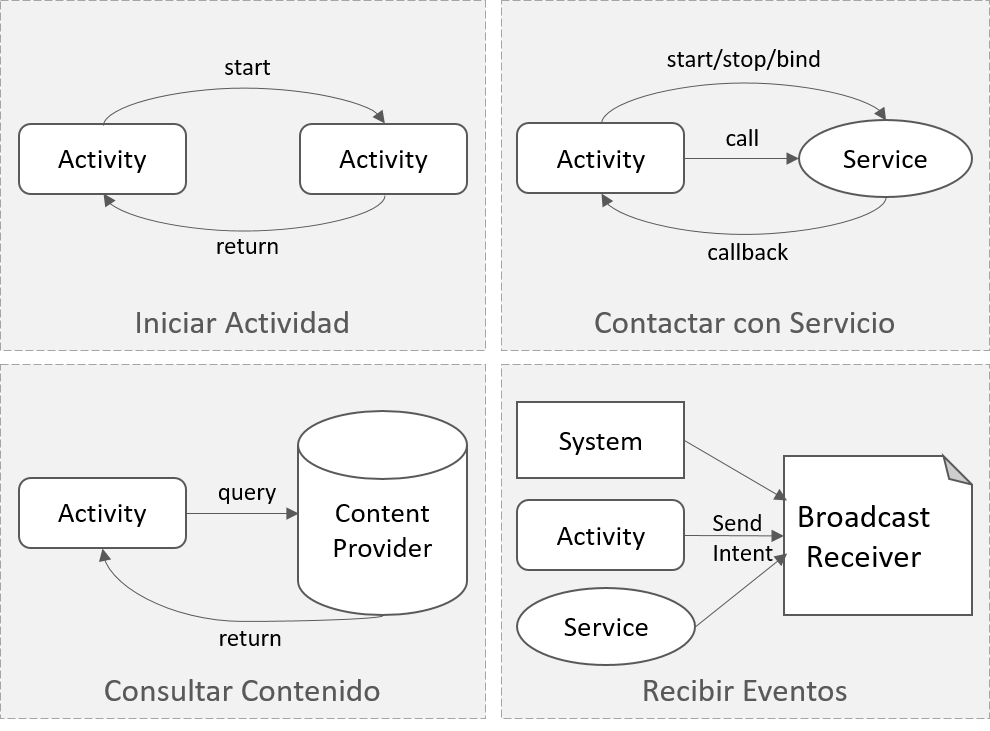
\includegraphics[width=1\columnwidth]{capitulo-5/graphics/mensajes_ipc}
\par\end{centering}
\caption[\emph{Framework Android}]{\label{fig5:mensajes-ipc}Marco de Trabajo \abbr{Android}}
\end{figure}

En la \figref{fig5:mensajes-ipc} se muestran las diferentes formas
de interacción entre los componentes \abbr{Android} citados anteriormente.
Como se puede apreciar, el mecanismo principal para todas las interacciones
son llevadas acabo por llamadas \abbr{IPC}. 

Una actividad se inicia por medio de un mensaje y puede lanzar otra
actividad en pantalla. Un servicio se inicia, se para y se asocia
por el mecanismo \abbr{IPC} como también las llamadas a métodos y
retorno de resultados son realizados por el mismo medio. Un proveedor
de contenidos es consultado con llamadas \abbr{IPC} y retorna los
resultados por el mismo medio. Todos los eventos son recibidos por
el receptor de mensajes por medio del \abbr{IPC}. Como es manifiesto
en la gráfica, el marco de trabajo de \emph{IPC Binder} se basa el
modelo \emph{Cliente-Servidor} (ver \ref{ssec52:criterios-dise=0000F1o})
y el patrón de diseño \emph{Proxy} \cite{Shalloway2004}.

\section{Arquitectura del proyecto}

\label{sec53:arquitectura}La solución presentada en este trabajo
puede describirse partiendo el mismo en tres componentes principales:
\begin{itemize}
\item \textbf{\emph{HARDroid}}: Es un servicio de reconocimiento de actividades
humanas específico para \abbr{Android}. Este componente tiene cabida
dentro de la capa de \emph{Application Framework} descrita en \ref{ssec52:tecnologia}
como un servicio utilitario. El algoritmo reconocedor de actividades
es un componente dinámico capaz de actualizar su clasificador continuamente.
\item \textbf{\emph{ActivitySurvey}}: Es una aplicación móvil de encuesta
que permite utilizar el servicio de reconocimiento y además evaluar
el resultado con el consentimiento del usuario. Este componente está
ubicado en la capa de \emph{Applications} descrita en \ref{ssec52:tecnologia}.
El resultado evaluado puede ser utilizado para mejorar el clasificador
de aprendizaje automático.
\item \textbf{\emph{Backend C4.5}}: Es un servicio web \abbr{REST} que
recolecta las evaluaciones del usuario que utiliza la aplicación de
encuesta. Además, almacena los resultados que surgen debido a la utilización
del reconocedor con el objetivo de crear el modelo de aprendizaje
automático de manera manual. 
\end{itemize}
\begin{figure}[H]
\begin{centering}
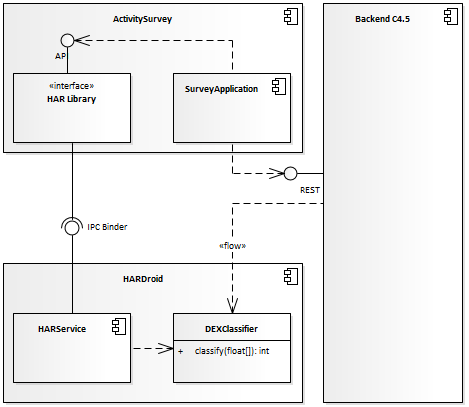
\includegraphics[width=0.8\columnwidth]{capitulo-5/graphics/arqui_general}
\par\end{centering}
\caption[Arquitectura del Proyecto]{\label{fig5:arqui-general}Arquitectura del Proyecto}

\end{figure}

En la \figref{fig5:arqui-general} se muestra la vista general de
la arquitectura del proyecto donde se muestran los dos aportes principales
de este trabajo junto con sus partes relevantes. El diagrama se describe
en lenguaje \abbr{UML} donde los componentes representan las aplicaciones
móviles distribuidas de manera independiente y un componente de servidor
para recolectar datos experimentales.

\section{HARDroid: Servicio de Reconocimiento}

\label{sec54:hardroid}El servicio \abbr{HARDroid} fue diseñado para
ajustarse a las características generales de los gestores y/o servicios
en la capa de \emph{Application Framework} de \abbr{Android}, Ej.
\emph{Location Manager} o \emph{Google Play Services}. La ventaja
del servicio \abbr{HARDroid} para las aplicaciones móviles hechas
por terceros es que aprovechan las últimas mejoras del motor de reconocimiento
de actividades, con actualización automática de la plataforma distribuida
como un \abbr{APK} independiente a través de la tienda \emph{Google
Play}. Esto permite a los usuarios estar actualizados y los desarrolladores
poseen mecanismos fáciles para integrarse al servicio \abbr{HAR}.

\begin{figure}[H]
\begin{centering}
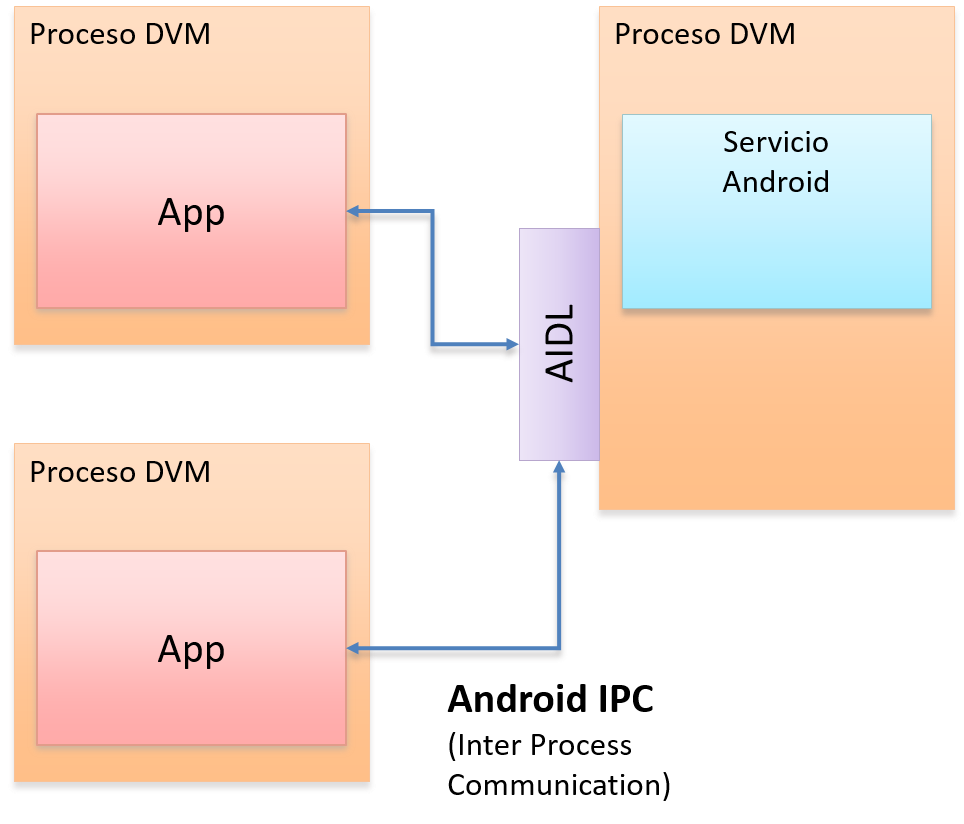
\includegraphics[width=0.8\columnwidth]{capitulo-5/graphics/hardroid_func}
\par\end{centering}
\caption[Servicio HARDroid]{\label{fig5:hardroid-func}Servicio \abbr{HARDroid}}

\end{figure}

En la \figref{fig5:hardroid-func} se muestra el esquema de funcionamiento
del servicio \abbr{HARDroid} en base al diseño expuesto en el párrafo
anterior. Este esquema de diseño es el más apropiado para crear aplicaciones
móviles distribuidas en \abbr{Android}, semejante a la arquitectura
de servicios de \emph{Google Play Services} \cite{Google2016l}. Las
aplicaciones móviles están confinadas en procesos separados del sistema
\abbr{Android}, cada cual en su entorno \abbr{DVM} correspondiente,
donde la comunicación entre procesos es llevado acabo por medio de
una interfaz \abbr{AIDL} parte del mecanismo \emph{IPC Binder} (ver
sección \ref{ssec52:framework}).

\subsection{Módulos Funcionales}

\label{ssec54:modulos}Desde el punto de vista conceptual el servicio
\abbr{HARDroid} puede ser dividido en cuatro módulos principales
que cumplen con las características específicas que se describen a
continuación.

\subsubsection{Interfaz de Servicio}

Este módulo define el modelo dominio y la interfaz del para integración
(a través de una \abbr{API}). En el dominio del problema se identificaron
los siguientes conceptos definidos:
\begin{itemize}
\item \emph{Cliente} (\texttt{\small{}ActivityRecognitionClient}): Un cliente
es un proceso remoto que requiere reconocer actividades humanas con
cierta periodicidad.
\item \emph{Conexión} (\texttt{\small{}ServiceConnection}):\emph{ }Es una
entidad que mantiene la información de estado del servicio como sesión
del cliente. Posee un ciclo de vida de conexión y cierre.
\item \emph{Actividad Humana} (\texttt{\small{}HumanActivity}): Es una entidad
que modela una actividad humana reconocida.
\item \emph{Vector Característico} (\texttt{\small{}Feature}): Es una entidad
que modela el conjunto de valores característicos utilizados durante
el procesamiento de la señal de los sensores.
\item \emph{Resultado de Reconocimiento} (\texttt{\small{}ActivityRecognitionResult}):
Es un conjunto de actividades humanas reconocidas junto con la precisión
estimada y los datos complementarios generados durante el calculo
en forma de vector característico.
\end{itemize}
En la \figref{fig5:domain-model} se muestra el diagrama de clases
con los artefactos construidos para el manejo del dominio del problema.
Las clases se definieron con semejanza a los conceptos de \emph{Google
Play Services} \cite{Google2016l} y la documentación se describe
en (véase \cite{GimenezYegros2016d}).

\begin{figure}[H]
\begin{centering}
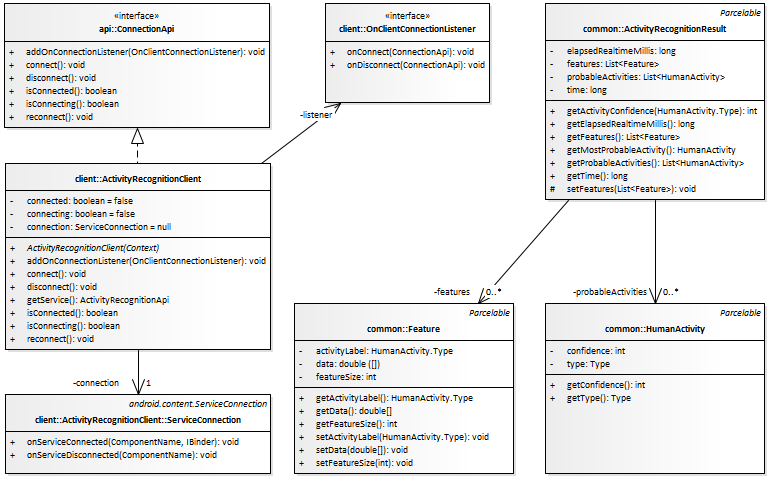
\includegraphics[width=1\columnwidth]{capitulo-5/graphics/class_domain}
\par\end{centering}
\caption[Diagrama de clases del dominio del problema]{\label{fig5:domain-model}Diagrama de clases del dominio del problema.}

\end{figure}

La interfaz del servicio se compone de un conjunto de llamadas para
que cualquier cliente pueda realizar con las siguientes acciones:
\begin{itemize}
\item \emph{Conectarse} al servicio
\item \emph{Desconectarse} del servicio
\item \emph{Subscribirse} estableciendo la periodicidad de los resultados
de actividades humanas esperados. 
\item \emph{Obtener} un resultado de actividades humanas al instante.
\end{itemize}
Teniendo en consideración el modelo de dominio citado anteriormente
y las acciones requeridas se presenta la interfaz proveída por el
servicio en la \figref{fig5:service-layer}.

\begin{figure}[H]
\begin{centering}
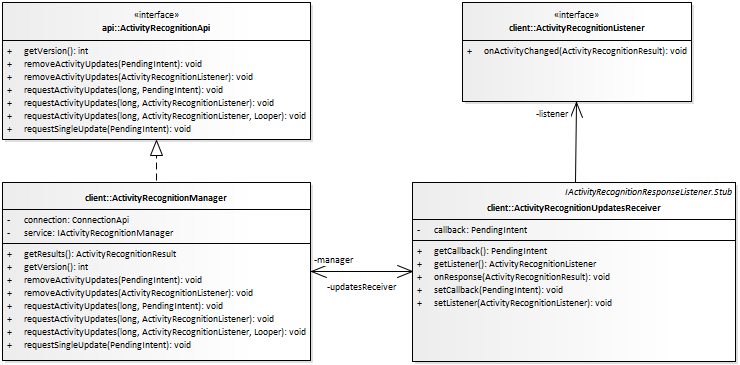
\includegraphics[width=1\columnwidth]{capitulo-5/graphics/class_service}
\par\end{centering}
\caption[Diagrama de clases de la capa de servicio]{\label{fig5:service-layer}Diagrama de clases de la capa de servicio.}

\end{figure}

Para poder clarificar la interfaz proveída por la capa de servicios
se describe textualmente el contrato definido para la \abbr{API}
para subscribirse a eventos de detección actividades humanas:
\begin{itemize}
\item \texttt{\footnotesize{}requestSingleUpdate(callbackIntent: PendingIntent): void
public} \\
Se subscribe a un evento de detección de actividad 
\item \texttt{\footnotesize{}requestActivityUpdates(detectionIntervalMillis: long,
}~\\
\texttt{\footnotesize{}listener: ActivityRecognitionListener): void
public}\\
Se suscribe a un evento de detección de actividad durante un intervalo
de mili-segundos. Espera la respuesta con un observador.
\item \texttt{\footnotesize{}requestActivityUpdates(detectionIntervalMillis: long,
}~\\
\texttt{\footnotesize{}callbackIntent: PendingIntent): void public}
\\
Se suscribe a un evento de detección de actividad durante un intervalo
de mili-segundos. Espera la respuesta con una función diferida.
\item \texttt{\footnotesize{}removeActivityUpdates(listener: ActivityRecognitionListener): void
public} \\
Se desuscribe a un evento de detección de actividad dado su observador.
\item \texttt{\footnotesize{}removeActivityUpdates(callbackIntent: PendingIntent): void
public}\\
Se desuscribe a un evento de detección de actividad dado su función
diferida.
\end{itemize}
En las siguientes secciones se detallan los módulos encargados de
implementar la lógica de negocio y funcionalidades bases de la interfaz
de servicio del motor reconocedor.

\subsubsection{Servidor}

Este módulo implementa las llamadas a procedimientos remotos desde
clientes distribuidos en otros procesos. La lógica del servicio esta
dividido en dos responsabilidades que manejan la conexión y la suscripción.
\begin{itemize}
\item \texttt{\small{}ActivityRecognitionService}: Es la función principal
del servicio ya que implementa el \abbr{IPC} de \abbr{Android} para
establecer la conexión con el cliente. Además se encarga de coordinar
las suscripción de clientes y publicar los resultados de detección
de actividades. 
\item \texttt{\small{}ActivityRecognitionManagerImpl}: Es un utilitario
que hace de mediador entre las llamadas remotas a la \abbr{API} de
la interfaz y la ejecución de la lógica del servicio.
\item \texttt{\small{}ActivityRecognitionSubscription}: Es una estructura
para memorizar las preferencias de suscripción de los clientes manejado
por la función principal del servicio.
\end{itemize}
La interacción que ocurre durante la conexión de un cliente al servidor
de reconocimiento se muestra en la \figref{fig5:service-subs}. Para
representar la interacción se utiliza un diagrama de secuencia \abbr{UML}
donde las clases en amarillo representan objetos en el proceso del
cliente, a través de la librería cliente \abbr{HARDroid}. Las clases
en azul son objetos en el proceso del servidor, a través de la aplicación
móvil \abbr{HARDroid}.

\begin{figure}[H]
\begin{centering}
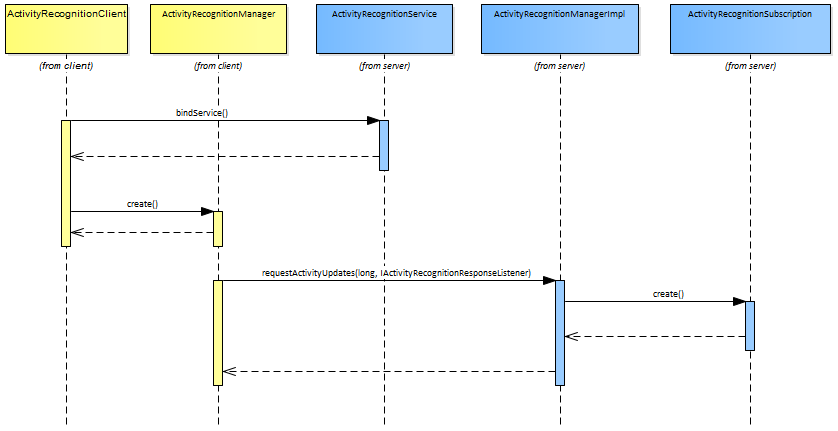
\includegraphics[width=1\columnwidth]{capitulo-5/graphics/service_subs}
\par\end{centering}
\caption[Interacción cliente y servidor de HARDroid]{\label{fig5:service-subs}Interacción cliente y servidor de \abbr{HARDroid}}
\end{figure}

El servidor mantiene una lista de suscripciones con los tiempos de
preferencia de notificación de eventualidad de cada cliente. 

\subsubsection{Procesamiento}

Este módulo se encarga de ejecutar el motor de reconocimiento de actividades
humanas a intervalos periódicos de tiempo siempre que hayan suscripciones
memorizadas. La ejecución del motor produce siempre un resultado global
de actividad humana.
\begin{itemize}
\item \texttt{\small{}ActivityRecognitionWorker}: Es la función principal
del motor de reconocimiento que programa una tarea periódica de recolección
de datos sensoriales, calculo de vectores característicos y clasificación
de actividad para producir y emitir un nuevo resultado.
\item \texttt{\small{}FeatureProcessing}: Es un utilitario que calcula los
vectores característicos.
\item \texttt{\small{}SignalProcessing}: Es un utilitario con funciones
de procesamiento de señales. 
\end{itemize}
La ejecución del motor de reconocimiento que empieza durante el inicio
del servidor de reconocimiento se muestra en la \figref{fig5:service-worker}.
El motor realiza las tareas en un intervalo de tiempo definido por
el menor tiempo memorizado en las suscripciones de clientes.

\begin{figure}[H]
\begin{centering}
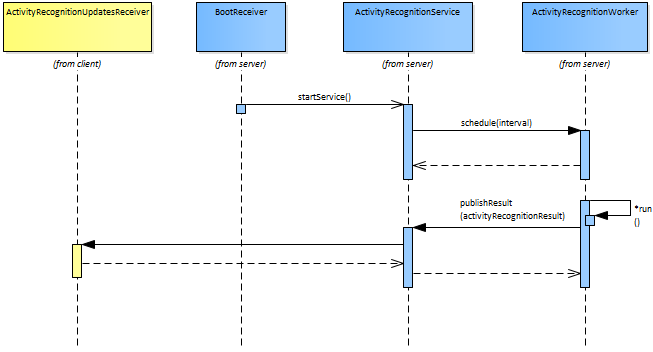
\includegraphics[width=1\columnwidth]{capitulo-5/graphics/service_worker}
\par\end{centering}
\caption[Procesamiento y publicación de resultados de HARDroid]{\label{fig5:service-worker}Procesamiento y publicación de resultados
de \abbr{HARDroid}}
\end{figure}

Ante la eventualidad de un nuevo resultado de reconocimiento emitido
por el motor de reconocimiento se realiza una publicación de resultados
a los clientes correspondientes. El algoritmo de reconocimiento se
describe a continuación.

\begin{algorithm}[H]
\begin{algorithmic}[1]
    \Require Conjunto de tiempos de subscripción de clientes $S$
	\Procedure{Reconocimiento}{$ S $}
		\If {$S \textit{ está vacio } $}
 			\State\textit{Terminar}
		\EndIf
		\State $t_w \leftarrow 10$
\rcomment{Esta es la ventana de tiempo necesaria para el reconocimiento}
		\State $t_{min} \leftarrow \min_{\forall s \in S} s$
		\State Esperar $t_{min} - t_w$ segundos 
		\State $ a_{xyz} = $ Leer datos de asceleracion por $t_w$ segundos o 512 muestras
		\State $ C = \emptyset$
		\For{$i := 1 \to 512$}
			\State $ v_f = $ Calcular vector caracteristicos de $a_{xyz}$ con valores entre $[i, i + 127]$
			\State $ c_a = $ Clasificar $v_f$ con el algoritmo \textit{C4.5}
			\State $ C = C \cup \{c_a\}$ 
			\State $i := i + 64$
        \EndFor
        \State $ M = $ Calcular matriz de confusión de $C$ 
		\State
		\Return $ M $
	\EndProcedure
\end{algorithmic}

\caption{\label{alg5:reconocimiento}Detección de actividades humanas}
\end{algorithm}


\paragraph{Clasificador}

Este módulo se encarga de la clasificación de un vector característico
y emite una estimación de la actividad humana detectada. Posee dos
implementaciones principales y complementarias.
\begin{itemize}
\item \texttt{\small{}ActivityClassifier}: Es una clase genérica que define
los métodos comunes de los clasificadores de actividades humanas.
\item \texttt{\small{}DecisionTreeClassifier}: Es la implementación de un
clasificador de actividades humanas basado en arboles de decisión
generados por el \emph{software} \texttt{\abbr{WEKA}} \cite{Frank2016}.
\item \texttt{\small{}DumbClassifier}: Es la implementación de un clasificador
de actividades humanas simple que no emite un resultado válido.
\item \texttt{\small{}DexModelLoader}: Es un utilitario para descargar de
Internet de manera segura un clasificador generado por \abbr{WEKA}.
El clasificador está implementado en una clase contenida en un artefacto
de \emph{software} en formato \abbr{JAR},
\end{itemize}
La actualización dinámica del modelo se muestra en la \figref{fig5:service-classi}.
Para la actualización al modelo clasificador más reciente generado
por medio de \abbr{WEKA} se depende de la conexión a Internet y un
recurso publicado remotamente. El mecanismo detallado se describe
en el apéndice \ref{chapB:carga-dinamica}.

\begin{figure}
\begin{centering}
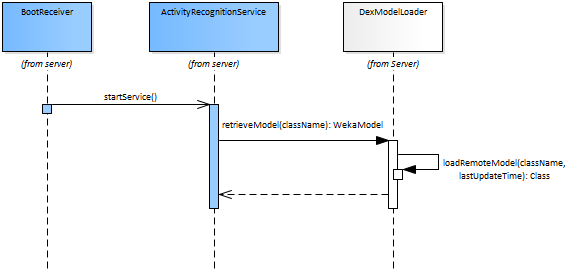
\includegraphics[width=1\columnwidth]{capitulo-5/graphics/service_classi}
\par\end{centering}
\caption[Actualización del clasificador WEKA]{\label{fig5:service-classi}Mecanismo de actualización del dinámica
del clasificador basado en \abbr{WEKA}}
\end{figure}


\section{ActivitySurvey: Encuesta de Evaluación}

\label{sec55:activity}Con el objetivo probar el funcionamiento del
servicio \abbr{HAR} en \abbr{Android} y evaluar los resultados producidos
al detectar las actividades realizadas por el usuario, se creó la
aplicación \emph{ActivitySurvey. }El diseño de la aplicación móvil
es bastante sencillo pero con los complementos necesarios que permitan
validar el funcionamiento de \abbr{HARDroid} y encuestar a los usuarios
finales durante una sesión de entrenamiento físico. En esta sección
se presenta la vista general de la aplicación explicada por medio
de artefactos que describen las funcionalidades básicas construidas. 

\subsection{Casos de Uso}

Las especificaciones funcionales describen el comportamiento de la
aplicación desde el punto de vista del usuario final. Los casos de
uso son:
\begin{itemize}
\item Registrarse
\item Responder Encuesta
\item Cambiar preferencias
\end{itemize}

\subsection{Diseño Detallado}

El diseño del proyecto se basa en los componentes comunes de una aplicación
móvil \abbr{Android} según lo expuesto en \ref{ssec52:framework}.
El diseño se compone de una colección desacoplada de Actividades,
Servicios, Proveedores y Receptores que se describen a continuación.

\subsubsection{Módulos Funcionales}
\begin{itemize}
\item \texttt{\small{}SurveyApplication}: Es el contexto de la aplicación
que mantiene acceso a las preferencias, los servicios y las suscripciones
a mensajes.
\item \texttt{\small{}FeedActivity}: Es la vista principal de la aplicación
que despliega la lista de actividades detectadas en una línea de tiempo
como tarjetas de preguntas. Cada pregunta puede ser obviada, corregida
o aseverada. 
\item \texttt{\small{}SettingsActivity}: Es la vista de configuración de
la aplicación que modifica las preferencias del usuario final y las
almacena en el dispositivo móvil.
\item \texttt{\small{}DetectorService}: Es un servicio que mantiene una
conexión persistente con el servicio \abbr{HAR}. El servicio es iniciado
o parado dependiendo de la necesidad del usuario en ser encuestado.
\item \texttt{\small{}DetectedActivitiesService}: Es un servicio de función
diferida que permite recibir actualizaciones de resultados detectados
por el servicio \abbr{HAR}. Por cada actividad humana detectada,
persiste la información y notifica por mensaje que existen nuevos
resultados.
\item \texttt{\small{}NotificationReceiver}: Es un receptor de mensajes
para crear alertas auditivas en el momento que se detectan nuevos
resultados. Sirven para avisar al usuario final que debe contestar
una nueva encuesta.
\item \texttt{\small{}HumanActivityFeed}: Es el proveedor de contenidos
que persiste los resultados a ser evaluados durante la encuesta.
\item \texttt{\small{}UpdateActionReceiver}: Es un receptor de mensajes
para sincronizar los resultados evaluados en la encuesta con el servidor
remoto de usuarios encuestados.
\end{itemize}
En la \figref{fig5:act-surv-diag} se muestran los módulos funcionales
que hacen a la aplicación con una notación en base a los componentes
comunes de \abbr{Android} y su interacción. 

\begin{figure}[H]
\begin{centering}
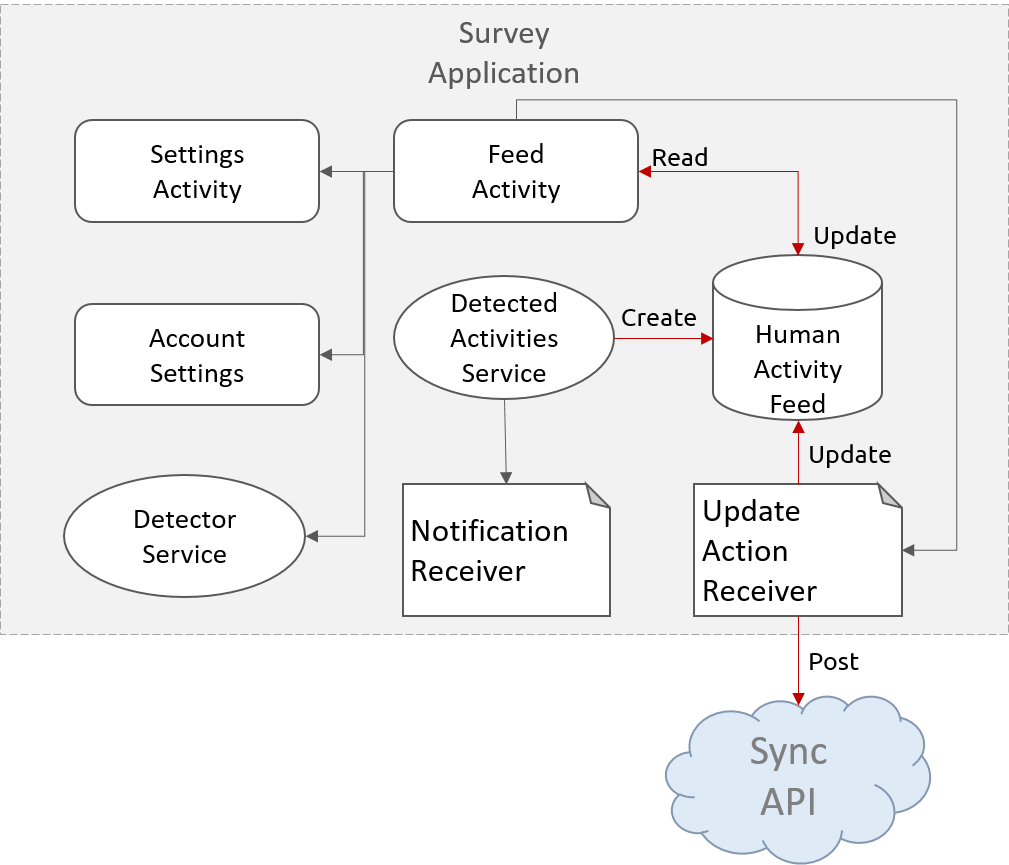
\includegraphics[width=1\columnwidth]{capitulo-5/graphics/act_surv_diag}
\par\end{centering}
\caption[Diagrama de diseño de ActivitySurvey]{\label{fig5:act-surv-diag}Diagrama de diseño de \emph{ActivitySurvey}}

\end{figure}


\paragraph{Persistencia}

Las actividades humanas detectadas durante una sesión deben ser almacenadas
en el teléfono móvil para luego transmitirlas a un servidor central.
Los resultados de cálculos del reconocedor y las encuestas respondidas
por los usuarios se persisten en una base de datos personal perteneciente
a la aplicación. El diagrama desplegado en la \figref{fig5:act-surv-er}
representa el modelo de datos utilizado. Esta información se sincroniza
por medio un servicio Web externo para un posterior análisis y mejoras
al algoritmo de clasificación.

\begin{figure}[H]
\begin{centering}
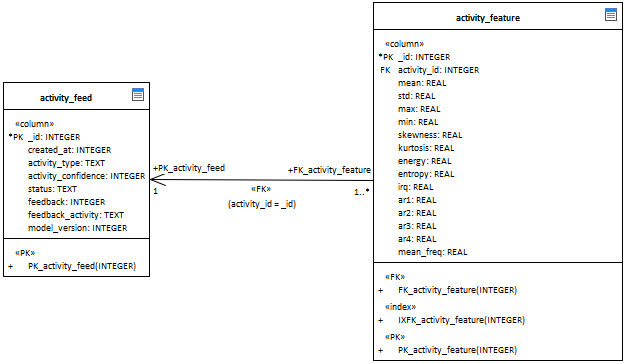
\includegraphics[width=1\columnwidth]{capitulo-5/graphics/act_surv_er}
\par\end{centering}
\caption[Modelo de datos de ActivitySurvey]{\label{fig5:act-surv-er}Modelo de datos de \emph{ActivitySurvey}}
\end{figure}


\subsubsection{Interfaz de Usuario}

En base al modelo de información se presentan los contextos que permiten
a los usuarios navegar y descubrir las vistas y acciones disponibles
en la aplicación móvil. El diagrama de navegación en la \figref{fig5:navega}
muestra la lista completa de pantallas necesarias para que los usuarios
interactúen con los datos. 

En la aplicación de encuesta, los usuarios tienen la capacidad de
ver sus actividades reconocidas, responder a la encuesta confirmando
la actividad o corrigiendo la misma. 

\begin{figure}
\begin{centering}
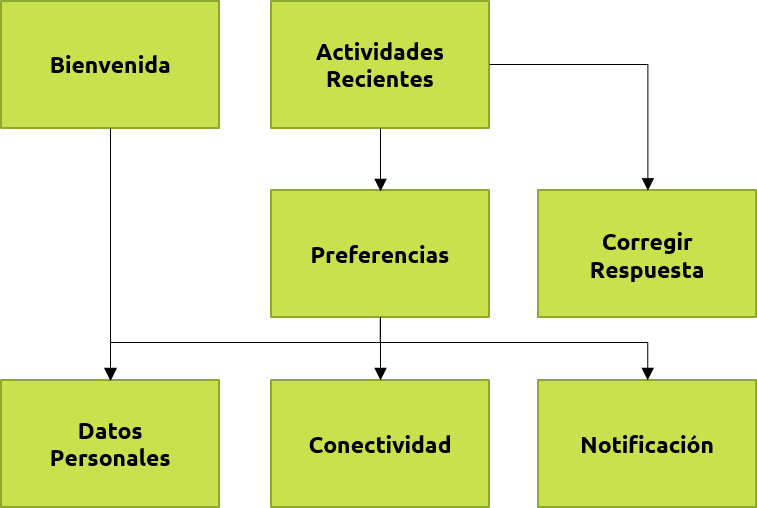
\includegraphics[width=1\columnwidth]{capitulo-5/graphics/navegacion}
\par\end{centering}
\caption[Mapa de navegación de pantallas de ActivitySurvey]{\label{fig5:navega}Mapa de navegación de pantallas de \emph{ActivitySurvey}}

\end{figure}

El diagrama de navegación de pantallas muestra la relación directa
entre pantallas por medio de cuadros y flechas. Una flecha que va
desde la pantalla \emph{Bienvenida} a otra pantalla \emph{Datos Personales}
ocurre por medio de una interacción del usuario en la pantalla \emph{Bienvenida}. 

\section{Conclusión}

\label{sec56:conclusion}En esta sección presentamos un servicio de
reconocimiento de actividades humanas (\abbr{HAR}) para la plataforma
\abbr{Android}. Está construido en base a las mejores prácticas de
servicios de utilitarios existentes de propiedad intelectual privada
como\emph{ Google Play Services}. Esta herramienta permite que aplicaciones
móviles desarrolladas por terceros no dependan de implementaciones
privativas sino de un componente de software libre. Bajo un modelo
colaborativo, cualquier solución que utilice esta alternativa obtiene
beneficios como adaptarlo a sus necesidades o gozar de las mejoras
evolutivas. 

Además, esta implementación fue probada por medio de una aplicación
móvil independiente donde se evaluó el funcionamiento desacoplado
proveído por el marco de trabajo de \abbr{Android}. Los resultados
obtenidos fueron satisfactorios en cuanto a la integración entre aplicación
móvil y servicio utilitario en procesos independientes. Los resultados
experimentales confirmaron que es posible recolectar información en
terreno a través de la aplicación de encuesta y luego esta información
pueda ser validada, limpiada y utilizada para mejorar el algoritmo
de clasificación basado en árboles de decisión de forma ininterrumpida.
Se requieren experimentación adicional para evaluar el servicio bajo
condiciones más realistas cuando el servicio es instalado en diferentes
teléfonos móviles y en interacción con otras aplicaciones distintas
para su evaluación.
